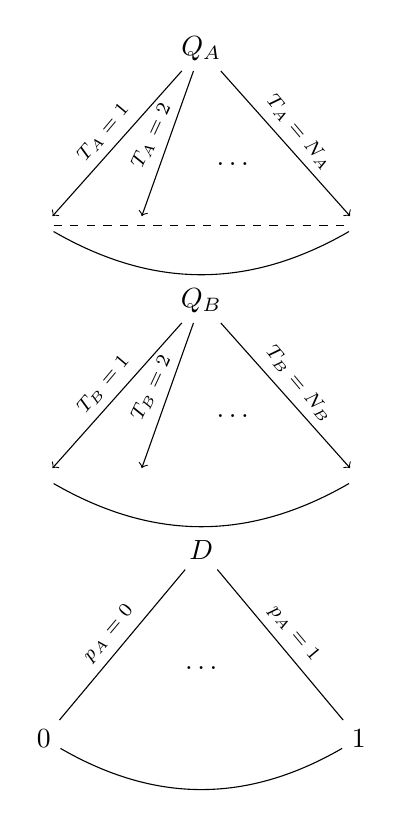
\begin{tikzpicture}[-, node distance = 2cm, scale=0.8]
    \node[anchor=north](QA){\(Q_A\)};
    \node[anchor=north](QA_d1) at (-2.5, -3) {};
    \node[anchor=north](QA_d2) at (-1, -3) {};
    \node[anchor=north](QA_d3) at (0.5, -2) {\(\dots\)};
    \node[anchor=north](QA_d4) at (2.5, -3) {};

    \path[->] (QA) edge node [above, rotate=50] {\scriptsize{\(T_A=1\)}}(QA_d1);
    \path[->] (QA) edge node [above, rotate=65] {\scriptsize{\(T_A=2\)}}(QA_d2);
    \path[<-] (QA_d4) edge node [above, rotate=310] {\scriptsize{\(T_A = N_A\)}}(QA);

    \path (QA_d1) [dashed] edge node {}(QA_d4);
    \path (QA_d1) [bend right] edge node {}(QA_d4);

    \node[anchor=north](QB) at (0, -4) {\(Q_B\)};
    \node[anchor=north](QB_d1) at (-2.5, -7) {};
    \node[anchor=north](QB_d2) at (-1, -7) {};
    \node[anchor=north](QB_d3) at (0.5, -6) {\(\dots\)};
    \node[anchor=north](QB_d4) at (2.5, -7) {};

    \path[->] (QB) edge node [above, rotate=50] {\scriptsize{\(T_B=1\)}}(QB_d1);
    \path[->] (QB) edge node [above, rotate=65] {\scriptsize{\(T_B=2\)}}(QB_d2);
    \path[<-] (QB_d4) edge node [above, rotate=310] {\scriptsize{\(T_B = N_B\)}}(QB);

    \path (QB_d1) [bend right] edge node {}(QB_d4);

    \node[anchor=north] (D) at (0, -8) {\(D\)};
    \node[anchor=north](D_d1) at (-2.5, -11) {0};
    \node[anchor=north](D_dots) at (0, -10) {\(\dots\)};
    \node[anchor=north](D_d2) at (2.5, -11) {1};

    \path[-] (D) edge node [above, rotate=50] {\scriptsize{\(p_A=0\)}}(D_d1);
    \path[-] (D_d2) edge node [above, rotate=310] {\scriptsize{\(p_A=1\)}}(D);

    \path (D_d1) [bend right] edge node {}(D_d2);

\end{tikzpicture}
